
Let us revisit the concentric data problem present in Figure \ref{fig:circle_data}, and compare the classification of LDA to KDA. As discussed, the data is not linearly separable and so we expect LDA to be a poor classifier. For LDA, we obtain the failed classification (Figure \ref{fig:LDA_circles}) and the projection vector along with the data in Figure \ref{fig:LDA_proj_circles}.
\\
\centerline{\begin{minipage}{0.6\textwidth}
    \begin{figure}[H]
    \centering
    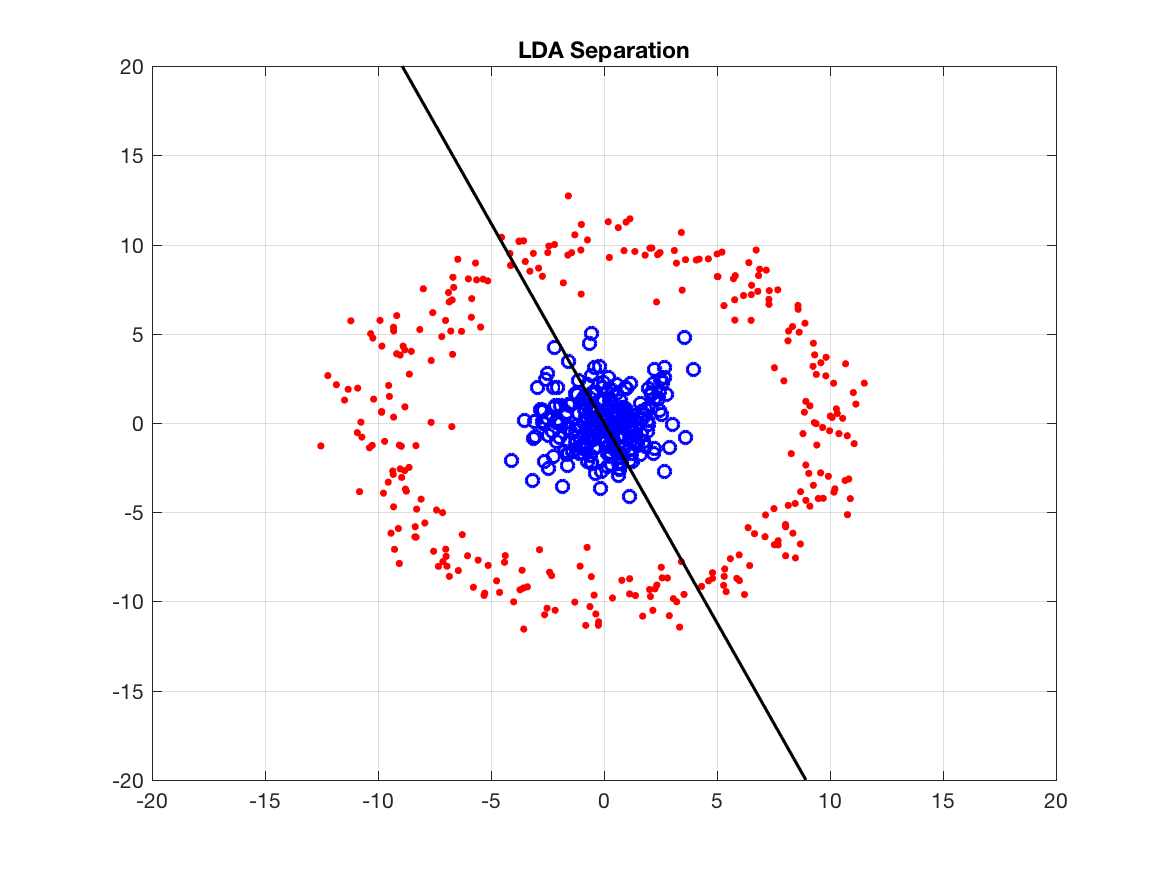
\includegraphics[trim={0cm 0cm 0cm 0cm},clip,width=1.0\columnwidth]{kda_test/LDA_circles}
    \caption{Figure \ref{fig:circle_data} data with LDA projection vector}
    \label{fig:LDA_circles}
    \end{figure}
\end{minipage}}
\centerline{\begin{minipage}{0.6\textwidth}
    \begin{figure}[H]
    \centering
    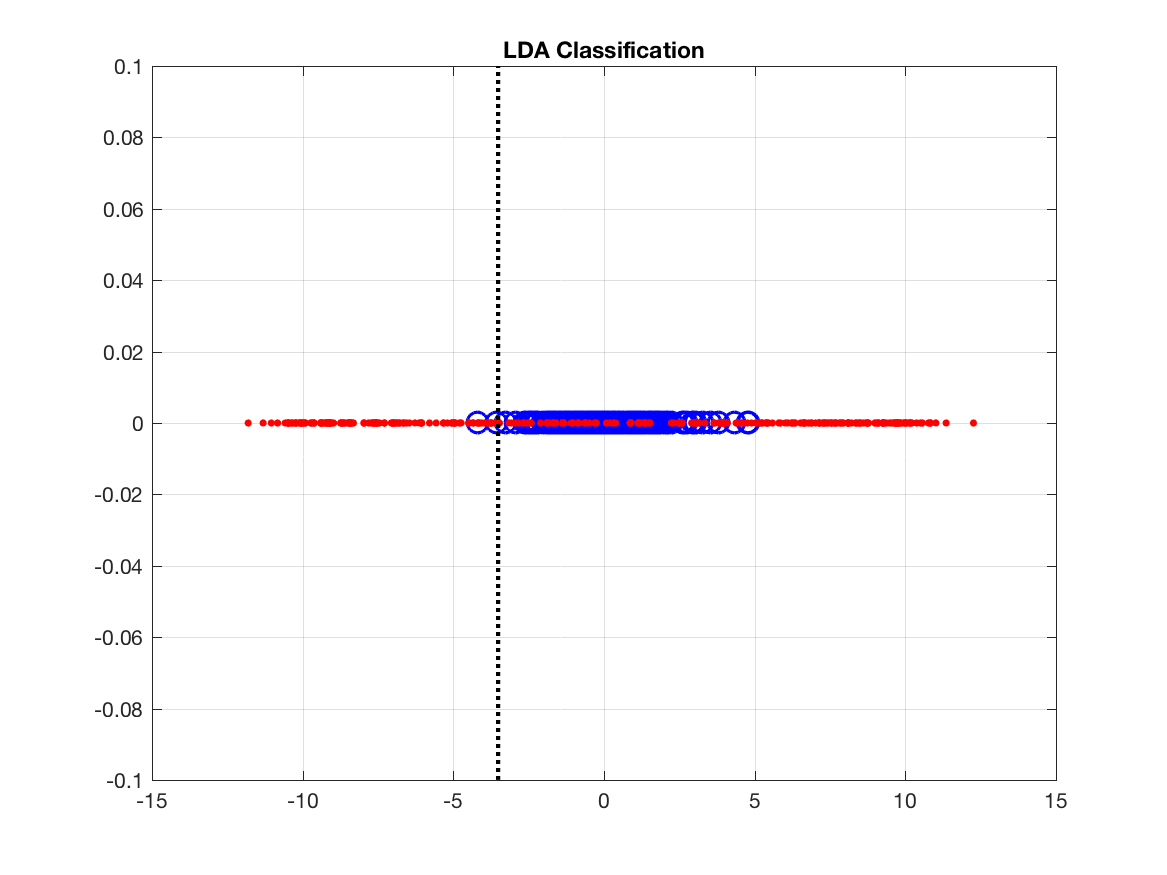
\includegraphics[trim={0cm 0cm 0cm 0cm},clip,width=1.0\columnwidth]{kda_test/LDA_proj_circles}
    \caption{Figure \ref{fig:circle_data} LDA classification}
    \label{fig:LDA_proj_circles}
    \end{figure}
\end{minipage}}
\\
\\
Because of the kernel trick, we cannot plot the projection ``vector" directly. Nonetheless, the successful classification is shown in Figure \ref{fig:KDA_proj_circles}.

\centerline{\begin{minipage}{0.8\textwidth}
    \begin{figure}[H]
    \centering
    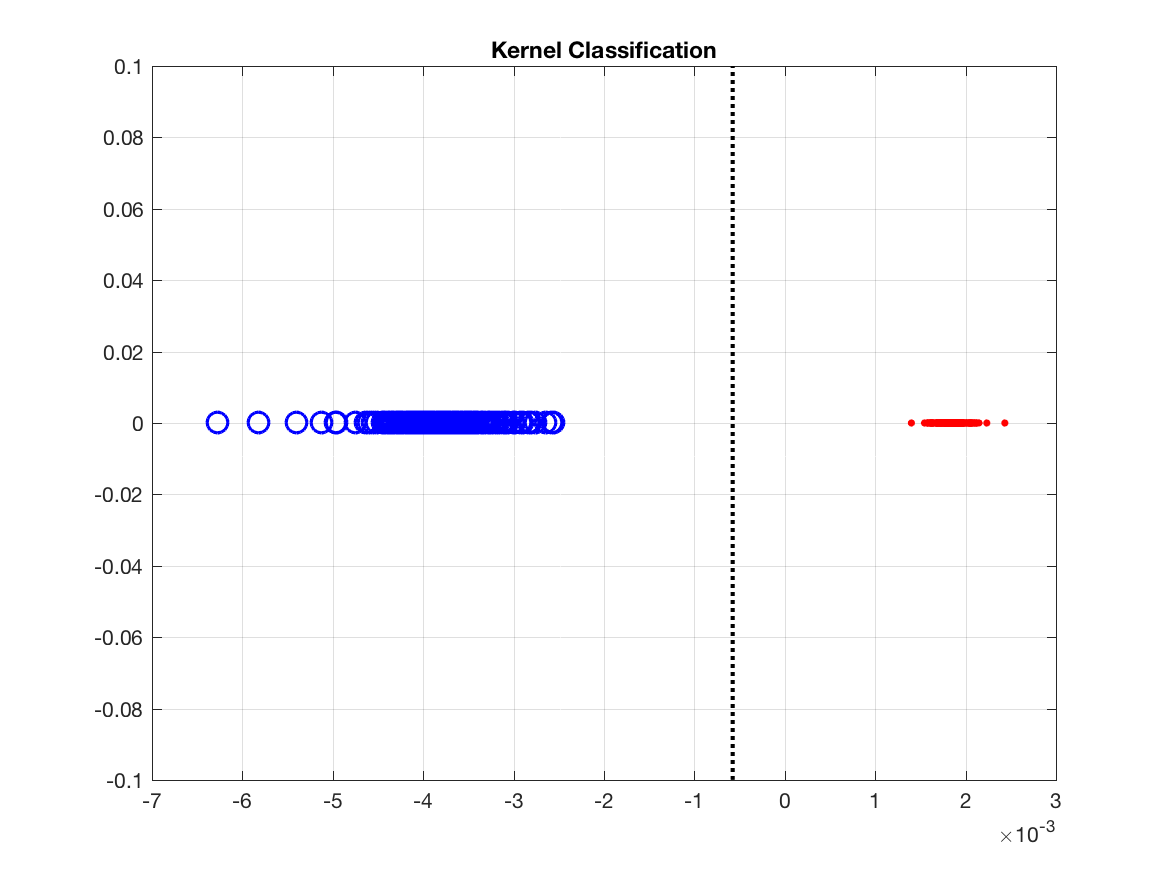
\includegraphics[trim={0cm 0cm 0cm 0cm},clip,width=0.8\columnwidth]{kda_test/KDA_proj_circles}
    \caption{Figure \ref{fig:circle_data} KDA classification}
    \label{fig:KDA_proj_circles}
    \end{figure}
\end{minipage}}
